\documentclass{ctexart}
\usepackage{PhysicalChemistryNote}

\begin{document}\pagestyle{plain}
\setcounter{footnote}{0}
\begin{center}
    \tbf{\Huge Chapter 2 热力学第一定律}
\end{center}\vspace{15pt}

如果你在第一章成功驯服了那群自由散漫的气体分子,那么恭喜——现在,你即将踏入热力学的核心战场,直面宇宙最公平的法则:能量守恒.%
是的,本章的主题可以用一句话概括:“能量不会消失,只会变着花样让你算到头秃.”

让我们先做个深呼吸(毕竟气体的体积变化你已了如指掌),然后思考一个灵魂问题:%
为什么你不能通过打开冰箱使得房间里更凉快?答案就在热力学第一定律的“铁三角”中:内能,功与热.它们的关系比你抽屉里的杂物还复杂,但数学表达却简单到令人怀疑人生——$\Delta U=Q+W$%
(注:公式的简洁程度与理解它的脑细胞死亡率成反比).

本章你将解锁以下成就:%
围观焦耳如何用搅拌水桶的执念证明“热与功是一家”;%
理解内能不是某种神秘内力,而是分子在微观层面集体狂欢的账单;%
发现迈尔医生一边给船员放血治坏血病,一边偷偷推演能量守恒的跨界操作;%
学会用系统与外界划分宇宙,从此理直气壮地把实验室爆炸归咎于“开放系统的不可控性”.

值得一提的是,本章的数学公式将比你的新年计划更守信用——它们绝不会凭空消失或无故增生.%
不过,符号规则可能会让你在功是正还是负的哲学问题中怀疑人生.(友情提示:小心在考试中上演负负得正的悲剧.)

最后,请牢记:热力学第一定律是宇宙的终极储蓄卡,能量可以转账,兑换,甚至分期付款,但余额永远不变.%
现在,就让我们一起走进这家银行,看一看存款规则吧.
\newpage
\documentclass{ctexart}
\usepackage{PhysicalChemistryNote}

\begin{document}\pagestyle{plain}
\noindent\tbf{\LARGE 2A 热力学的基本概念\footnote{本节的前两部分内容偏经验化和理论化,也没有严格的论证以支撑,在逻辑上可能也有不周之处,敬请谅解.}}\vspace{15pt}\\
\indent 热力学(Thermodynamics,源自古希腊语$\theta\ep\rho\mu o\varsigma$和$\delta\upsilon\nu\alpha\mu\iota\varsigma$),是研究热现象中物态转变和能量转换规律的学科.%
它着重研究物质的平衡状态以及与准平衡态的物理和化学过程.广义地说,热力学是研究系统宏观性质变化和系统状态变化的科学,它回答了一个过程能否发生的问题.\vspace{12pt}\\
\Section{2A.1 系统}
\Part{系统是热力学研究的对象}
\indent 我们进行科学研究时,需要确定所研究的对象,把研究的物质与其余分开(这一分隔可以是实际存在的,也可以是你假想的).我们对研究对象做如下定义.
\begin{definition}[2A.1.1 系统与环境]
    \tbf{系统}是人为划定的研究对象(以前也称为\tbf{体系}),而在系统外与系统密切相关且影响所能及的部分则称为\tbf{环境}\footnotemark.
\end{definition}
\footnotetext{你也可以简单地理解为除系统之外的其余部分.}
系统可以是一个反应容器,一台发动机,你的一个细胞,一杯水……你可以发现,系统和环境之间有时候是完全隔离的,有时候则不是.%
根据系统与环境之间的关系,我们可以对系统进行如下分类.
\begin{definition}[2A.1.2 系统的分类]
    根据系统与环境之间的关系,我们可以把系统分成如下三类.
    \begin{enumerate}[label=\tbf{\arabic*.}]
        \item \tbf{隔离系统}:系统完全不受环境的影响,和环境没有物质或能量的交换;又称为\tbf{孤立系统}.
        \item \tbf{封闭系统}:系统与环境没有物质交换,但可以有能量交换.
        \item \tbf{敞开系统}:系统与环境既可以有能量交换又可以有物质交换.
    \end{enumerate}
\end{definition}
敞开系统在我们的研究中提到的较少,而隔离系统和封闭系统是我们重点关注的研究对象.\vspace{4pt}\\
\Part{过程,途径和平衡态}
\indent 世界是变化的,系统也是变化的.
\begin{definition}[2A.1.3 过程与途径]
    给定系统的两个状态,记为始态和终态.在一定环境条件下,系统发生由始态到终态的变化,则称系统发生了一个\tbf{热力学过程},简称\tbf{过程(process)}.\\
    系统从始态到终态的变化可以由一个或者多个步骤进行,这些步骤被称作\tbf{途径(path)}.
\end{definition}
按照始态,终态的性质和过程中环境的性质,可以将过程大致分为如下几类.
\begin{definition}[2A.1.4 常见的过程]
    常见的过程有如下几类.
    \begin{enumerate}[label=\tbf{\arabic*.}]
        \item \tbf{等温过程}:系统在过程中保持温度不变,且等于恒定的环境温度.
        \item \tbf{等压过程}:系统在过程中保持压力不变,且等于恒定的环境压力.
        \item \tbf{等容过程}:系统在过程中保持的体积不变.\\
            刚性密闭容器内发生的过程一般都是等容过程.
        \item \tbf{绝热过程}:系统在过程中与环境没有热的交换,或因变化太快而来不及与环境热交换.\\
            带绝热壁的容器内的过程,或者爆炸过程,都可以视作\tbf{绝热过程}.
    \end{enumerate}
\end{definition}
一般来说,经过足够长的时间,系统总会达到一个稳定的状态,这一稳定状态下我们才能描述系统的各项性质(否则它们总是处于不断的变动中).因此,我们需要定义\tbf{平衡态}.
\begin{definition}[2A.1.5 热力学平衡状态]
    当系统的所有性质都不随时间而改变时,称系统处于\tbf{热力学平衡状态}.此时的系统须满足如下条件.
    \begin{enumerate}[label=\tbf{\arabic*.}]
        \item \tbf{热平衡}:系统各部分的温度相等.
        \item \tbf{力平衡}:系统各部分没有不平衡的力存在.
        \item \tbf{相平衡}:当系统有多个相时,物质在各相之间的分布达到平衡,相间没有物质的净转移.
        \item \tbf{化学平衡}:如果系统内各物质发生化学反应,那么达到平衡后系统的物质组成不随时间而改变.
    \end{enumerate}
\end{definition}
在本章(乃至热力学这一整个部分)我们都主要讨论平衡态(或者近平衡态)的系统.对于非平衡态的系统,我们将在之后讨论.\vspace{4pt}\\
\Part{系统的性质}
\indent 我们通常用系统的宏观可测性质(例如体积,压力,温度,物质的量,表面张力等等)%
来描述系统的热力学状态.这些性质称为\tbf{热力学变量}.根据热力学变量的性质,我们可以将其分为两类.
\begin{definition}[2A.1.5 热力学变量的分类]
    根据是否具有加和性,可以将系统的热力学变量分为如下两类.
    \begin{enumerate}[label=\tbf{\arabic*.}]
        \item \tbf{广度性质}:又称为\tbf{容量性质},其数值与系统的规模成正比.广度性质具有加和性,即系统的某种广度性质等于这系统各部分的这种广度性质的总和.
        \item \tbf{强度性质}:其数值与系统的规模无关,不具有加和性(例如,你不能把两杯$50\tccentigrade$的水混在一起并宣称现在它们是$100\tccentigrade$的).
    \end{enumerate}
\end{definition}
常见广度性质有物质的量,质量,热力学能\footnote{我们将在\tbf{2B}中提到热力学能的概念.}等;常见强度性质有压力,温度,密度,黏度等等.\\
\indent 回顾我们在\tbf{1A.1}中提到的状态函数,是为了描述系统的状态而存在的.因此,同一个状态的系统应当对应一个固定的状态函数值,%
而不论它是由什么途径得到的.因此,我们给出状态函数的严格定义.
\begin{definition}[2A.1.6 状态函数]
    处于平衡状态的热力学系统,若其宏观物理量具有确定的值,并且这些物理量仅由系统所处的状态所决定,与达到平衡态的过程无关,我们就称这一物理量为系统的\tbf{状态函数}.
\end{definition}\vspace{8pt}
\Section{2A.2 热平衡,热力学第零定律和热}
\indent 我们在\tbf{1A}中给出了温度的粗浅的定义,现在我们详细地再次论述这一概念.\\
\indent 温度的概念最初源于人类对冷热现象的直观感知.在日常生活中,人们通过触觉区分物体的“冷”与“热”,%
例如感知火焰的灼热,冰雪的寒冷,或通过观察自然现象(如水结冰或沸腾)推测环境温度的变化.%
古代文明已尝试量化冷热程度,例如中国汉代用“炭火变色”判断冶炼温度,古希腊通过混合冷热水调节沐浴温度.%
然而,这些方法依赖主观感受或经验观察,缺乏普适性和精确性.\\
\indent 17世纪后,随着温度计的发明,温度的测量逐渐脱离主观感知,成为基于物质热膨胀性质的客观物理量.%
例如,水银温度计通过液柱长度变化反映温度差异,首次将冷热程度转化为可量化,可复现的数值.这一工具的发展促使科学家追问温度的本质,%
最终通过热力学与统计力学的理论框架,将生活中的“冷热”抽象为描述系统热运动强度的物理量——温度.\\
\indent 我们不禁要问:为什么温度计能测定温度呢?这就要从它的原理——\tbf{热平衡}开始讲起.
\begin{definition}[2A.2.1 热平衡]
    当两个或多个热力学系统通过导热壁(允许热量传递的界面)接触时,若它们的宏观性质在长时间后不再发生任何变化,则称这些系统达到了\tbf{热平衡}.此时,系统间的净热流量为零,但微观粒子仍存在动态的能量交换.
\end{definition}
那么,温度计是如何判定温度相等的呢?换句话说,如果它和两个不同物体都建立了热平衡,这两个物体之间是否也能建立平衡呢?大量实验事实表明,热平衡具有递推性.
\begin{theorem}[2A.2.2 热力学第零定律]
    若两个热力学系统均与第三个系统处于热平衡状态,此两个系统也必互相处于热平衡.
\end{theorem}
热力学第零定律不能通过任何理论上的推导得出,这是一条类似数学中的公理的定律.\\
\indent 在我们的设想中,建立了热平衡的两个系统必定有一个相等的状态函数,我们就定义这一状态函数为\tbf{温度}.%
简而言之,如果两个系统建立了热平衡,那么它们的温度相等.%
热力学第零定律的实质是指出了温度这一状态函数的存在,并且给出了一种比较温度的方法.%
在比较各个系统的温度时,不需要将它们互相接触,只需将一个作为标准的第三系统分别于各个系统接触达到热平衡即可.%
这个作为标准的第三系统就是\tbf{温度计}.\\
\indent 人们对于热的本质的认识进行了长时间的探寻,一段时间内错误的“热质说”也甚嚣尘上.%
经由我们在\tbf{1B}中对温度的统计学概念的讨论,我们知道温度可以衡量微观分子做无规则运动的强度(实际上是平动能).%
当温度不同的系统接触时,应当通过分子的碰撞交换能量.经由这种方式交换的能量就是\tbf{热}.
\begin{definition}[2A.2.3 热]
    \tbf{热}是由于温度不同而在系统与环境之间交换或传递的能量,用符号$Q$表示.\\
    当系统吸热时,$Q$取正值,即$Q>0$;系统放热时,$Q$取负值,即$Q<0$.
\end{definition}
\begin{hint}
    热力学中的最基本的概念,即温度和热量,常常难以界定的十分妥帖.人们为了先有温度再有热量还是先有热量再有温度争论了许久.\\
    一种观点认为,应该先引入温度的概念,然后定义热量为两个不同温度的系统接触时传递的能量;%
    另一种观点认为,应该首先讨论热平衡(即宏观上没有热量的流动),然后定义温度为两个处于热平衡的系统所共有且相等的状态函数.%
    应当说,温度和热量是两个相互依存的物理量,它们之间在逻辑上是循环的关系.\\
    不过,你也许应当把主要的精力放在研究热力学的基本原理和将它们应用于解决化学中的实际问题,%
    而非刻意追求形式逻辑上的圆满.毕竟这不是数学,而我们的理论已经能相当好地描述这个世界了.
\end{hint}
\vspace{8pt}
\Section{2A.3 功}
\Part{功的定义}
\indent 你也许在初中物理中已经学过机械功,电功等等关于功的概念.在热力学中,功的定义如下.
\begin{definition}[2A.3.1 功]
    除了热以外以其它各种形式传递的能量称为\tbf{功},用符号$W$表示.\\
    系统对外做功时,$W$取负值,即$W<0$;环境对系统做功时,$W$取正值,即$W>0$.
\end{definition}
\begin{hint}
    有别于我们提到的各种状态函数,功和热都是依赖于途径的.%
    因此,为了以示区别,功和热对应的小量改用$\delta$表示,而非其它状态函数所用的微分符号$\di$.
\end{hint}
一般来说,各种形式的功都是广度量和强度量的乘积.%
例如机械功是位移$\di x$与力$F$的乘积,即
\[\delta W=F\di x\]
而电功是电势差$E$与电荷量$\di Q$的乘积,即
\[\delta W=E\di Q\]
等等.强度量决定了能量的传递方向,广度量决定了功的大小.\\
\indent 宏观地看,功是大量质点以有序运动而传递的能量,热是大量质点以无序运动传递的能量.\vspace{4pt}\\
\Part{膨胀功}
\indent 气体的膨胀会对外界做功,这是机械功的一种简单的体现.%
设想气体存放在带活塞(与器壁之间无摩擦)的容器中,容器横截面积为$A$.设气体压力为$p_\i$,外界压力为$p_\e$\footnote{此处的$\i$和$\e$分别指internal和external,用于表示内压和外压.}.%
当$p_\i>p_\e$时,气体就会向外膨胀,对外界做功.%
设活塞移动的距离为$\dx$,于是气体做的膨胀功$\delta W$为
\[\delta W=-F_\e\dx=-\left(\dfrac{F_\e}{A}\right)(A\dx)=-p_\e\di V\]
需要注意的是,由于气体是对环境做功,因此计算力$F$时应当计算外界对活塞的压力(你可以想象活塞上放了一个重物,重物对活塞的压力为$F_\e$,那么气体膨胀的力将用于抬升该重物,该力与抬升距离的乘积就是气体所做的功).\\
\indent 根据膨胀过程中外压的不同,我们可以对其做如下分类.
\begin{definition}[2A.3.2]
    我们大致将气体的膨胀分为如下几类.
    \begin{enumerate}[label=\tbf{\arabic*.}]
        \item \tbf{自由膨胀}:外压$p_\e$恒为$0$,即气体向真空膨胀.
        \item \tbf{恒外压膨胀}:外压$p_\e$恒为一定值.
        \item \tbf{准静态膨胀}\footnotemark :外压$p_\e$保持比内压$p_\i$大一个无穷小量$\di p$.
    \end{enumerate}
\end{definition}
\footnotetext{此处的(以及本节之后的)准静态膨胀是指等温条件下的准静态膨胀.我们在\tbf{2C}中还会看到绝热条件下的准静态膨胀.}
\indent 假定我们研究的气体是理想气体.现在,我们逐一推导在上述几种过程下气体从体积$V_1$膨胀到$V_2$时所做的功.
\begin{derivation}
    \begin{enumerate}[label=\tbf{\arabic*.}]
        \item 自由膨胀时,我们有
            \[W=\int_{V_1}^{V_2}0\di V=0\]
            这表明气体自由膨胀时不对外做功.
        \item 对抗恒外压膨胀时,我们有
            \[W=\int_{V_1}^{V_2}-p_\e\di V=-p_\e\left(V_2-V_1\right)\]
            如果气体发生了多次恒外压膨胀,那么只需分别计算即可.
        \item 我们首先考虑气体体积变化为无穷小量$\di V$时,气体做的功
            \[\delta W=-p_\e\di V=-\left(p_\i+\di p\right)\di V\]
            注意到其中有一个二阶无穷小量$\di p\di V$,可以忽略(通俗地来说,你可以认为$\di p\ll p_\i$,因此可以忽略不计),%
            于是积分可得
            \[W=\int_{V_1}^{V_2}-p_\i\di V=\int_{V_1}^{V_2}-\dfrac{nRT}{V}\di V=-nRT\ln\dfrac{V_2}{V_1}\]

    \end{enumerate}
\end{derivation}
如果我们观察$p-V$图像,就可以发现准静态膨胀是同一过程下系统做功最大的途径.\\
当我们将$p-V$曲线下的矩形取得足够细时,系统压力$p_\i$和环境压力$p_\e$差别足够小而可以忽略,此时众多的矩形的面积之和%
(根据定积分的定义)就等于$p-V$曲线下围的面积,也就是准静态膨胀所做的功.除此之外的任何一种膨胀方式,所做的功均小于等于该曲线下围的面积.
\begin{figure}[H]
    \centering\documentclass{standalone}
\usepackage{PhysicalChemistryNote}
\begin{document}
\begin{tikzpicture}
    \filldraw[lightgray] (0.3,0)--(0.3,1/3.3)--(3.3,1/3.3)--(3.3,0)--(0.3,0);
    \draw[->] (0,0) -- (4,0) node[right]{$V$};
    \draw[->] (0,0) -- (0,3.5) node[above]{$p$};
    \draw[domain=0.3:3.3] plot[smooth](\x,1/\x);
    \draw[dashed] (0.3,1/0.3) -- (0.3,0) node[below]{$V_1$};
    \draw[dashed] (3.3,1/3.3) -- (3.3,0) node[below]{$V_2$};
    \draw[dashed] (0.3,1/3.3) -- (3.3,1/3.3) node[right]{$p_\e$};
\end{tikzpicture}
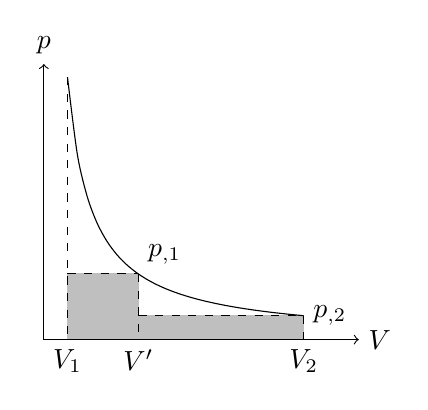
\begin{tikzpicture}
    \filldraw[lightgray] (0.3,0)--(0.3,1/1.2)--(1.2,1/1.2)--(1.2,1/3.3)--(3.3,1/3.3)--(3.3,0)--(0.3,0);
    \draw[->] (0,0) -- (4,0) node[right]{$V$};
    \draw[->] (0,0) -- (0,3.5) node[above]{$p$};
    \draw[domain=0.3:3.3] plot[smooth](\x,1/\x);
    \draw[dashed] (0.3,1/0.3) -- (0.3,0) node[below]{$V_1$};
    \draw[dashed] (3.3,1/3.3) -- (3.3,0) node[below]{$V_2$};
    \draw[dashed] (1.2,1/1.2) -- (1.2,0) node[below]{$V'$};
    \draw[dashed] (0.3,1/1.2) -- (1.2,1/1.2) node[above right]{$p_{\e,1}$};
    \draw[dashed] (1.2,1/3.3) -- (3.3,1/3.3) node[right]{$p_{\e,2}$};
\end{tikzpicture}
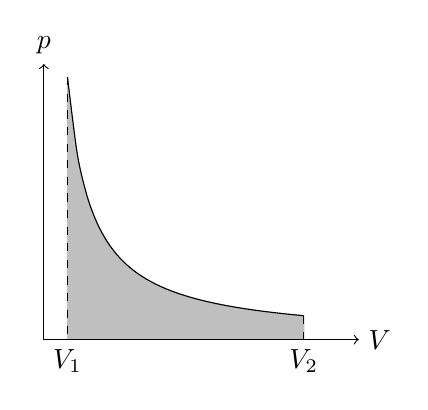
\begin{tikzpicture}
    \filldraw[lightgray] (0.3,0)--plot[domain=0.3:3.3,smooth](\x,1/\x)--(3.3,0);
    \draw[->] (0,0) -- (4,0) node[right]{$V$};
    \draw[->] (0,0) -- (0,3.5) node[above]{$p$};
    \draw[domain=0.3:3.3] plot[smooth](\x,1/\x);
    \draw[dashed] (0.3,1/0.3) -- (0.3,0) node[below]{$V_1$};
    \draw[dashed] (3.3,1/3.3) -- (3.3,0) node[below]{$V_2$};
\end{tikzpicture}
\end{document}
\end{figure}
\indent 由此可见,即使始态和终态一样,过程中做的功$W$也会随着途径的改变而改变.%
因此,功不是状态函数,它与变化的途径有着密切的联系.同样地,热也具有这样的性质.%
我们不能说系统中含有多少功或热,只能在具体的变化过程中求出功和热.\vspace{4pt}\\
\Part{压缩功}
\indent 与膨胀功类似,当气体被压缩时,环境对气体做功.我们来看以下三种对气体做功的方式.
\begin{figure}[H]
    \centering\input{picture/CompressionWork.tex}
\end{figure}
可以发现,准静态压缩所做的功是最小的,而一次性恒外压压缩所做的功是最大的.\vspace{12pt}\\
\Section{2A.4 准静态过程和可逆过程}
\Part{准静态过程}
\indent 我们已经在\tbf{2A.3.2}中提到了准静态膨胀.现在,我们对准静态过程进行较为严谨的定义.
\begin{definition}[2A.4.1 准静态过程]
    如果在一个过程的每个瞬间,系统都接近于平衡状态,其状态函数在系统的各部分都有确定的取值,整个系统可以看成一系列极接近平衡的状态构成,这样的过程被称作\tbf{准静态过程}.
\end{definition}
在准静态膨胀中,不论何时内外压仅相差一个无穷小量$\di p$,可以近似地看作内外力平衡,因而是准静态过程.\\
\indent 准静态过程在实际上是办不到的(你不可能让一个系统在变化的同时时刻保持平衡),但当一个过程进行地很慢时,这个过程就趋近于准静态过程.\vspace{4pt}\\
\Part{可逆过程}
\indent 考虑我们在上面提到的准静态膨胀和准静态压缩过程,你可以发现膨胀时系统对环境做的功恰好等于压缩时环境对系统做的功.%
换句话说,如果你把膨胀时做的功收集起来(例如转化为重力势能)并再次压缩,那么系统将复原.\\
\indent 然而,如果你采取了其它的膨胀方式,就会发现无论如何你不能用膨胀所做的功再将其压缩回原来的状态.%
如果你执意这么做,就会发现环境发生了不可逆的变化:它向系统做功,自己得到热\footnote{关于功和热转化的不可逆性,我们将在\tbf{Chapter 3}中讨论.}.\\
\indent 显然,准静态膨胀和压缩是特殊的,经过准静态膨胀后可以在不造成任何影响的情况下将系统和环境复原.这是一种在热力学中极为重要的过程,即\tbf{可逆过程}.
\begin{definition}[2A.4.2 可逆过程]
    \tbf{可逆过程}是指过程发生后能够被复原并对系统本身或外界不产生任何影响的过程;%
    另一种定义是系统能够在无能量损失或耗散的情形下通过无穷小的变化实现反转的热力学过程.\\
    反之,如果采取任何方法都不能使系统和环境复原,就称为\tbf{不可逆过程}.\\
    如果这一过程是一个循环的过程,那么系统和环境将恢复初始态而没有任何变化,称这样的过程为\tbf{可逆循环}.
\end{definition}
很多实际过程都可以视作可逆过程,例如液体在沸点的蒸发,可逆电池在外加电动势和电池电动势近似相等时的充电和放电,等等.\\
\indent 以后我们将会知道,可逆过程是能量利用效率最高的过程.
\end{document}
\newpage
\documentclass{ctexart}
\usepackage{PhysicalChemistryNote}

\begin{document}\pagestyle{plain}
\noindent\tbf{\LARGE 2B 热力学第一定律}\vspace{15pt}\\
\indent “退休后打算做什么?”\\
\indent “去当博物馆保安,看守‘永动机原型机’——反正它们永远不需要充电.”\\
\indent “那是个空壳子啊喂!”\vspace{12pt}\\
\Section{2B.1 热力学第一定律}
\Part{内能}
\indent 一块烧红了的铁和一块常温下安静地躺在地面上的铁,相信你对它们蕴含的能量大小肯定有一个依赖于直觉的判断.%
在热力学中,“物质蕴含的能量”有一个准确的定义——\tbf{内能}.
\begin{definition}[2B.1.1 内能]
    系统的总能量称为\tbf{内能},又称为\tbf{热力学能},记为$U$.\\
    通常,系统的内能是系统内所有粒子的动能与势能之和.
\end{definition}
需要说明的是,系统总体的动能和势能并不包含在内能之中.你携带在高铁上的咖啡\footnote{原稿为可乐,但考虑到可乐中的CO$_2$容易逸出造成内能改变,因此改为咖啡.}%
和在家里喝的咖啡虽然速度不同,但是内能是相同的;同样,这罐咖啡的内能也不会因为你把它带到山上就发生改变.%
不过,要是你有兴趣加热或者冰镇这瓶咖啡,它的内能自然就会发生改变.\\
\indent 我们需要指出下一事实.
\begin{theorem}[2B.1.2 内能的性质]
    内能是状态函数.
\end{theorem}
这不难理解,毕竟无论经历怎样的改变,只要系统的状态确定,其中粒子的运动情况和相互作用就是确定的,内能也就是确定的.\vspace{4pt}\\
\Part{热力学第一定律}
\indent 热力学第一定律的诞生与人类对“永动机”的追求密切相关.%
自中世纪起,许多人试图设计无需外部能量输入的机械(如利用重力,浮力或磁力的“自驱动机”),但均以失败告终.%
18世纪末,工业革命推动了对蒸汽机效率的研究,科学家逐渐意识到热,功与能量之间存在深层联系.\\
\indent 大量事实(例如Joule做的精确测定热功当量的实验)表明,能量不会凭空产生或消失,只会以不同的形式发生转化.这就是我们熟知的\tbf{能量守恒定律}.\\
\indent 能量守恒定理表明,一个孤立系统的总能量不会发生改变(这一系统不与环境发生能量或物质的交换,因而它的能量不会增加或减少).%
考虑到我们研究的体系的总能量一般指内能(通常你也不会让它整体做奇怪的运动),因此我们就有\tbf{热力学第一定律}.
\begin{theorem}[2B.1.3 热力学第一定律]
    隔离系统的内能是守恒的.其数学形式为
    \[\Delta U=Q+W\text{\ \ \ 或\ \ \ }\di U=\delta Q+\delta W\]

\end{theorem}
我们将在接下来的很多地方用到热力学第一定律.不过,在此之前,我们先引入一些别的状态函数以更好地描述系统.\vspace{12pt}\\
\Section{2B.2 焓与热容}
\Part{焓}
\indent 假定系统在变化过程中不做其余功,则根据热力学第一定律有
\[\Delta U=Q+W\]
如果系统的变化是等容过程,那么$W=0$,于是
\[\Delta U=Q\]
如果系统的变化是等压过程,那么不妨设压力保持为$p$,则有
\[W=-p\left(V_2-V_1\right)\]
即
\[U_2-U_1=Q-pV_2+pV_1\]
移项可得
\[Q=\left(U_2+pV_2\right)-\left(U_1+pV_1\right)\]
这告诉我们,等压过程下系统的热量变化等于始态和终态的$(U+pV)$之差.这促使我们定义一个新的状态函数以更好地描述等压过程.
\begin{definition}[2B.2.1 焓]
    \tbf{焓}是定义为$U+pV$的状态函数,记为$H$.
\end{definition}
上面的推导告诉我们,在没有其它功的情况下,等容过程中的热$Q_V$全部用于系统热力学能$U$的增加,而等压过程中的热$Q_p$全部用于系统焓的增加.%
尽管我们不知道$U$和$H$的具体值,却可以通过测量上面两种过程中的热效应来衡量过程中的内能变化$\Delta U$或焓变$\Delta H$.\\
\indent 由于化学反应更常见的是恒压反应,因此在处理化学问题时,焓也许更加常用.\vspace{4pt}\\
\Part{热容}
\indent 我们知道,使不同的系统升高相同的温度,需要提供的热也不同.在阳光照射下的沙滩,你会明显感觉沙子的温度比海水要高.%
因此,物质吸收热而升高温度的能力是不同的,这促使我们定义\tbf{热容}以定量地表述这种能力.
\begin{definition}[2B.2.2 热容]
    \tbf{热容}的定义是系统升高单位热力学温度时吸收的热,记为$C$,即
    \[C=\dfrac{\delta Q}{\di T}\]
    显然,热容与物质的量有关,因此定义\tbf{摩尔热容}为
    \[C_\m=\dfrac{C}{n}=\dfrac1n\dfrac{\delta Q}{\di T}\]

\end{definition}
我们已经知道,在等压和等容过程中,分别有
\[\delta Q_V=\di U\ \ \ \ \ \delta Q_p=\di H\]
\indent 因此可以定义\tbf{定压热容}和\tbf{定容热容}.
\begin{definition}[2B.2.3 定压热容和定容热容]
    定压热容$C_p$和定容热容$C_V$分别定义为
    \[C_p=\dfrac{\delta Q_p}{\di T}=\pa HTp\ \ \ \ \ C_V=\dfrac{\delta Q_V}{\di T}=\pa UTV\]
    以及与\tbf{2B.2.2}类似地,也可以定义\tbf{定压摩尔热容}$C_{\text p,\m}$和定容摩尔热容$C_{V,\m}$.
\end{definition}
有了上述两种热容,我们就可以计算等压过程中的焓变和等容过程中的内能变,即
\[\Delta H=\int_{T_1}^{T_2}C_p\di T\ \ \ \ \ \Delta U=\int_{T_1}^{T_2}C_V\di T\]
其中$T_1,T_2$分别为始态和终态的温度.\\
\indent 热容是温度的函数,这意味着它也可以做如下的展开
\[C_{p,\m}=a+bT+cT^2+\cdots\ \ \ \ \ C_{V,\m}=a'+b'T+c'T^2+\cdots\]
实际计算中也常常用到这类展开式以求更精确的计算.
\end{document}
\newpage
\documentclass{ctexart}
\usepackage{PhysicalChemistryNote}

\begin{document}\pagestyle{plain}
\noindent\tbf{\LARGE 2C 热力学第一定律对气体的应用}\vspace{15pt}\\
\indent 作者很懒,于是什么都没留下.向各位征集导言.\vspace{12pt}\\
\Section{2C.1 热力学第一定律对理想气体的应用}
\Part{理想气体的$U$和$H$}
\indent Gay-Lussac和Joule分别独立完成了真空膨胀实验.%
他们在水浴的容器中添加一块隔板,一边充入高压气体,另一边抽成真空.随后,撤掉挡板,气体向真空膨胀.%
水浴内的温度计显示温度没有变化,因此这个过程满足$Q=W=0$,因此热力学能$U$没有变化.我们将从这一实验结果推出一个重要的推论.
\begin{derivation}
    对于定量的理想气体,其内能$U$可以用$p,V,T$三个变量中的两个进行表示.\\
    假如我们选择$T,V$作为$U$的变量,对$U$全微分可得
    \[\di U=\pa UTV\di T+\pa UVT\di V\]
    根据上述实验结果,有
    \[\di U=0\ \ \ \ \ \di T=0\ \ \ \ \ \di V\neq0\]
    于是
    \[\pa UVT=0\]
    换用$p,T$作为$U$的变量,同理可得
    \[\pa UpT=0\]
    这表明温度一定时,理想气体的$U$不随$p,V$的改变而改变.
    又因为
    \[\pa HVT=\pa{(U+pV)}VT=\pa UVT+\pa{pV}VT\]
    而对于定量的理想气体,温度一定时有$pV=nRT=\text{定值}$,于是$\pa {pV}VT=0$,从而
    \[\pa HVT=0\]
    同理可得
    \[\pa HpT=0\]
    这表明温度一定时,理想气体的$H$也不随$p,V$的改变而改变.
\end{derivation}
\begin{theorem}[2C.1.1 Joule定律]
    理想气体的热力学能和焓都是仅以温度为自变量的函数,与压力和体积无关,即
    \[U=U(T)\ \ \ \ \ H=H(T)\]

\end{theorem}
我们可以从分子动理论进行简单的解释:热力学能是分子的动能与相互作用的势能的总和.对于理想气体,动能仅与温度有关,%
而分子之间的相互作用力被忽略,即没有相互作用的势能这一项,因此其热力学能仅与温度有关.
\begin{hint}
    严格来讲,Gay-Lussac和Joule的实验并不精确,因为水的热容很大,一点小的热量变化也不会使温度发生明显改变.%
    不过,我们仍然可以通过外推$p\to0$的情形来说明Joule定律的合理性.\\
    在学习\tbf{Chapter 3}之后,我们可以根据Maxwell关系式来确证Joule定律的合理性.可以证明
    \[\pa UVT=T\pa pTT-p\ \ \ \ \ \pa HpT=V-T\pa VTp\]
    对于理想气体有$pV=nRT$,代入上式可得
    \[\pa UVT=\pa HpT=0\]
    而
    \[\pa UpT=\pa UVT\pa VpT=0\ \ \ \ \ \pa HVT=\pa HpT\pa pVT=0\]
    于是$U,H$均不随$p$和$V$的改变而改变.
\end{hint}
\Part{理想气体的$C_p$和$C_V$}
\indent 考虑到
\[C_p=\pa UTV\ \ \ \ \ C_V=\pa HTp\]
于是理想气体的定容热容也是仅与温度有关的函数.\\
\indent 对于等压过程,气体除了吸收热量升温之外,还要多吸收一部分热量膨胀对外做功,因此$C_p$总是比$C_V$大.%
我们现在来求两者的差值.
\setcounter{equation}{0}
\begin{derivation}
    首先考虑对于所有系统的普适情况.\\
    对于一个一般的系统,我们有
    \begin{equation}
        \begin{aligned}
            C_p-C_V
            &= \pa HTp-\pa UTV =\pa{(U+pV)}Tp-\pa UTV \\
            &= \pa UTp+p\pa VTp-\pa UTV
        \end{aligned}
    \end{equation}
    考虑$U$作为$V,T$的函数和$V$作为$p,T$的函数,即
    \[U=U(V,T)\ \ \ \ \ V=V(p,T)\]
    根据复合函数的链式求导法则有
    \begin{equation}
        \pa UTp=\pa UTV+\pa UVT\pa VTp
    \end{equation}
    将(2)代入(1)中可得
    \begin{equation}
        C_p-C_V=p\pa VTp+\pa UVT\pa VTp=\left[p+\pa UVT\right]\pa VTp
    \end{equation}
    上式就是一般气体的定压热容与定容热容之差的公式.对于理想气体,又有
    \begin{equation}
        \pa UVT=0\ \ \ \ \ \pa VTp=\dfrac{nR}{p}
    \end{equation}
    将(4)代入(3)可得
    \begin{equation}
        C_p-C_V=nR
    \end{equation}
    或
    \begin{equation}
        C_{p,\m}-C_{V,\m}=R
    \end{equation}

\end{derivation}
于是,我们得到了以下重要定理.
\begin{theorem}[2C.1.2 气体的$C_p$与$C_V$之差]
    对于一般的气体有
    \[C_p-C_V=\left[p+\pa UVT\right]\pa VTp\]
    对于理想气体有
    \[C_p-C_V=nR\text{\ \ \ 或\ \ \ }C_{p,\m}-C_{V,\m}=R\]

\end{theorem}
在以后,你也许会经常遇到要使用$C_p$或$C_V$却只给出了另外一种数据的情形,此时\tbf{2C.1.2}就将发挥它的作用.\vspace{4pt}\\
\Part{理想气体的绝热过程}
\indent 绝热过程是化学反应中的常见过程.对于气体的绝热膨胀,由于向外界做功的同时不能从外界吸收热,%
于是根据热力学第一定律可知气体的内能减小,温度必然降低.我们在此先讨论理想气体的绝热过程.
\begin{derivation}
    在绝热过程中,$Q=0$.在不做非膨胀功的情况下,我们有
    \[\di U=\delta W=-p\di V\]
    对$U$做全微分有
    \[\di U=\pa UTV\di T+\pa UVT\di V=C_V\di T\]
    由于理想气体满足$p=\dfrac{nRT}{V}$,于是代入有
    \[-\dfrac{nRT}{V}\di V=C_V\di T\]
    即
    \[\dfrac{\di T}{T}+\dfrac{nR}{C_V}\dfrac{\di V}{V}=0\]
    我们已经知道$C_p-C_V=nR$.令\tbf{热容比}$\gamma=\dfrac{C_p}{C_V}$,则有
    \[\dfrac{\di T}{T}+(\gamma-1)\dfrac{\di V}{V}=0\]
    如果$C_V$与温度无关(我们将来会知道对于理想气体,其热容确实是常数),那么上述式子积分可得
    \[TV^{\gamma-1}=\text{常数}\]
    将$T=\dfrac{pV}{nR}$代入上式可得
    \[pV^\gamma=\text{常数}\]

\end{derivation}
因此,我们可以得到理想气体绝热过程中满足的条件.
\begin{theorem}[2C.1.3 理想气体的绝热过程]
    理想气体从$T_1$变化至$T_2$的绝热过程满足
    \[W=\int_{T_1}^{T_2}C_V\di T=C_V\left(T_2-T_1\right)\]
    且
    \[p_1V_1^\gamma=p_2V_2^\gamma\]

\end{theorem}
在实际情况下,气体的变化一般介于等温过程和绝热过程之间,此时有%
$pV^\beta=\text{常数}(1<\beta<\gamma)$.这种过程被称为\tbf{多方过程}.\vspace{12pt}\\
\Section{2C.2 Carnot循环\footnote{音译为“卡诺循环”.}}
\indent 自从蒸汽机被发明以来,人们一直利用热机做功而应用于生产生活.
\begin{definition}[2C.2.1 热机]
    \tbf{热机}是能够将热源提供的一部分热量转化成为对外输出的机械能的机器.\\
    一般的热机由\tbf{高温热源}\footnotemark,\tbf{低温热源},\tbf{工作系统}构成,%
    在热源和工作系统之间用来进行能量传递和转化的媒介叫做\tbf{工作物质}.
\end{definition}
\footnotetext{热源是具有恒定温度且温度不随吸收或放出热量而发生的系统.}
\indent 19世纪初,蒸汽机的效率很低,只有3\%到5\%,大量的能量被浪费.%
热机工程师们望从理论上找出提高热机效率的办法.1824年,年轻的法国工程师N.L.S.Carnot设计了一个由两个等温过程和两个绝热过程构成的最简单的理想循环,后来被称为Carnot循环.%
这一热力学循环的提出为提高热机效率指明了方向,为推动热力学理论的发展做出了重要贡献.\vspace{4pt}\\
\Part{Carnot循环}
\indent 我们先介绍Carnot设计的循环过程.
\begin{figure}[H]
    \centering\documentclass{standalone}
\usepackage{PhysicalChemistryNote}
\begin{document}
\begin{tikzpicture}
    \draw[->] (0,0) -- (5,0) node[right]{$V$};
    \draw[->] (0,0) -- (0,5) node[above]{$p$};
    \draw[domain=1.0400:2.6207] plot[smooth](\x,4/\x);
    \draw[domain=2.6207:4.1602] plot[smooth](\x,{12*sqrt(2)/(\x^2.5)});
    \draw[domain=1.6510:4.1602] plot[smooth](\x,2/\x);
    \draw[domain=1.0400:1.6510] plot[smooth](\x,{3*sqrt(2)/(\x^2.5)});
    \coordinate[label=above:{$A\left(p_1,V_1,T_\h\right)$}] (1) at (1.0400,3.8460);
    \coordinate[label=above right:{$B\left(p_2,V_2,T_\h\right)$}] (2) at (2.6207,1.5263);
    \coordinate[label=right:{$C\left(p_3,V_3,T_\c\right)$}] (3) at (4.1602,0.4807);
    \coordinate[label={[xshift=-0.4cm,yshift=-0.85cm]$D\left(p_4,V_4,T_\c\right)$}] (4) at (1.6510,1.2114);
    \node[circle,fill,inner sep=1pt] at (1) {};
    \node[circle,fill,inner sep=1pt] at (2) {};
    \node[circle,fill,inner sep=1pt] at (3) {};
    \node[circle,fill,inner sep=1pt] at (4) {};
\end{tikzpicture}
\end{document}
\end{figure}
\begin{definition}[2C.2.2 Carnot循环]
    以$n\mol$理想气体为工作物质,温度为$T_\h$的高温热源和温度为$T_\c$的低温热源作为能量来源,进行如下四个步骤.
    \begin{enumerate}[label=\tbf{\arabic*.}]
        \item \tbf{等温可逆膨胀}\\
            系统与高温热源$T_\h$接触,作等温可逆膨胀,由状态$A\left(p_1,V_1,T_\h\right)$变为状态$B\left(p_2,V_2,T_\h\right)$.
        \item \tbf{绝热可逆膨胀}\\
            系统离开热源,作绝热可逆膨胀,由状态$B\left(p_2,V_2,T_\h\right)$变为状态$C\left(p_3,V_3,T_\c\right)$.
        \item \tbf{等温可逆压缩}\\
            系统与高温热源$T_\c$接触,作等温可逆压缩,由状态$C\left(p_3,V_3,T_\c\right)$变为状态$D\left(p_4,V_4,T_\c\right)$.
        \item \tbf{绝热可逆压缩}\\
            系统离开热源,作绝热可逆压缩,由状态$D\left(p_4,V_4,T_\c\right)$变为状态$A\left(p_1,V_1,T_\h\right)$.
        \end{enumerate}
\end{definition}
接下来,我们来推导Carnot循环中各步骤的功和热,以计算整个循环的效率.
\begin{derivation}
    \begin{enumerate}[label=\tbf{\arabic*.}]
        \item 等温可逆膨胀时$\Delta U_1=0$,且$\displaystyle W_1=-\int_{V_1}^{V_2}=nRT_\h\ln\dfrac{V_1}{V_2}$,于是$Q_\h=-W_1=nRT_\h\dfrac{V_2}{V_1}$.
        \item 绝热可逆膨胀时$Q=0$,则$\displaystyle W_2=\Delta U_2=\int_{T_\h}^{T_\c}C_V\di T$.
        \item 等温可逆压缩时$\Delta U_3=0$,且$\displaystyle W_3=-\int_{V_3}^{V_4}=nRT_\c\ln\dfrac{V_3}{V_4}$,于是$Q_\c=-W_3=nRT_\c\dfrac{V_4}{V_3}$.
        \item 绝热可逆压缩时$Q=0$,则$\displaystyle W_4=\Delta U_4=\int_{T_\c}^{T_\h}C_V\di T$.
    \end{enumerate}
    由于\tbf{2.}和\tbf{4.}均为绝热过程,根据\tbf{2C.1.3}可知
    \[T_\h V_2^{\gamma-1}=T_\c V_3^{\gamma-1}\ \ \ \ \ T_\c V_4^{\gamma-1}=T_\h V_1^{\gamma-1}\]
    于是
    \[\dfrac{V_1}{V_2}=\dfrac{V_4}{V_3}\]
    于是
    \[W_{\text{tot}}=W_1+W_2+W_3+W_4=nRT_\h\ln\dfrac{V_1}{V_2}+nRT_\c\ln\dfrac{V_3}{V_4}=nR\left(T_\h-T_\c\right)\ln\dfrac{V_1}{V_2}\]
    \[Q=-W=nR\left(T_\h-T_\c\right)\ln\dfrac{V_2}{V_1}\]

\end{derivation}
于是我们有
\begin{theorem}[2C.2.3 Carnot循环的功和热]
    系统完成一次\tbf{2C.2.1}所示的Carnot循环,做的总功为
    \[W=nR\left(T_\h-T_\c\right)\ln\dfrac{V_1}{V_2}\]
    从高温热源吸收的热$Q_\h$为
    \[Q_\h=nRT_\h\ln\dfrac{V_2}{V_1}\]
    向低温热源放出的热$Q_\c$为
    \[Q_\c=nRT_\c\ln\dfrac{V_1}{V_2}\]

\end{theorem}
\Part{热机效率}
\indent 热机从高温热源吸热$Q_\h$,仅将一部分转化为功,将另一部分热$Q_\c$传递给低温热源.%
我们可以定义\tbf{热机效率}来衡量热机将吸收的热转化为功的比例.
\begin{definition}[2C.2.4 热机效率]
    将热机对环境做的功$W$和从高温热源吸收的热$Q_\h$之比称为\tbf{热机效率},记为$\eta$.    
\end{definition}
\setcounter{equation}{0}
对于Carnot热机有
\begin{equation}
    \eta=\dfrac{-W}{Q_\h}=\dfrac{nR\left(T_\h-T_\c\right)\ln\dfrac{V_2}{V_1}}{nRT_\h\ln\dfrac{V_2}{V_1}}=\dfrac{T_\h-T_\c}{T_\h}=1-\dfrac{T_\c}{T_\h}
\end{equation}
\begin{equation}
    \eta=\dfrac{-W}{Q_\h}=\dfrac{Q_\c+Q_\h}{Q_\h}=1+\dfrac{Q_\c}{Q_\h}
\end{equation}
因此,Carnot热机的效率$\eta<1$.我们将在\tbf{Chapter 3}中证明所有工作于$T_\h$和$T_\c$的热机的效率都不可能超过Carnot热机,从而所有热机的效率都小于$1$.\vspace{4pt}\\
\Part{制冷机与热泵}
\indent 如果把Carnot热机沿$A-D-C-B-A$的途径倒开,就得到了一个制冷机.此时,环境对系统做功,系统从低温热源吸收热量$Q_\c'$,向高温热源放出热量$Q_\h'$.%
与热机相似的,我们可以定义制冷效率.
\begin{definition}[2C.2.5 制冷效率]
    将制冷机从低温热源吸收的热量$Q_\c'$与环境对系统做的功$W$之比称为\tbf{制冷效率},记为$\beta$.
\end{definition}
对于Carnot热机有
\[\beta=\dfrac{Q_\c'}{W}=\dfrac{T_\c}{T_\h-T_\c}\]
\indent 对于制冷机,我们关注的是通过做功使得从低温热源中吸收热量.%
对于热泵,虽然它的本质是和制冷机相同的,不过我们更关心它向高温热源输送的热量.同样地,我们有热泵的工作效率.
\begin{definition}[2C.2.6 热泵的工作效率]
    将热泵向高温热源放出的热量$Q_\h'$与环境对系统做的功$W$之比称为\tbf{热泵的工作效率},记为COP.
\end{definition}
对于Carnot热机有
\[COP=\dfrac{Q_\h'}{W}=\dfrac{T_\h}{T_\h-T_\c}\]
\indent 一般的商用热泵的COP在$2$到$7$之间,说明做$\SI{1}{J}$的功可以向高温热源输送$\SI{2}{J}$到$\SI{7}{J}$热能.%
这比直接用这些功转化为热量要高效得多.\vspace{12pt}\\
\Section{2C.3 热力学第一定律对实际气体的应用}
\Part{Joule-Thomson效应}
\indent 前面已经指出,Joule所做的自由膨胀实验并不精确.因此,在1853年,他与Thomson合作完成了\tbf{节流膨胀实验}.\\
\indent 节流膨胀实验在一段内部装有多孔塞(或节流阀)\footnote{Joule也许采用的是棉花或者软木塞.}的绝热管道中进行.将气体通入管道的一端,并调节该侧气体的压力恒定为$p_1$.%
随后,气体缓慢流经多孔塞,由于多孔塞的局部阻力,气体压力降低至$p_2$.%
经过一段时间达到稳定态后,入口和出口的气体温度各自稳定在$T_1$和$T_2$.这一过程被称为\tbf{节流膨胀过程}.
\begin{derivation}
    我们假定体积为$V_1$的气体经过上述节流膨胀后的体积变为$V_2$.\\
    后来的气体对这气体做等温压缩,压力为$p_1$,体积由$V_1$变化至$0$,做的功为
    \[W_1=-p_1\Delta V=p_1V_1\]
    气体从多孔塞出来后等温膨胀,对前面的气体做功,压力为$p_2$,体积由$0$变化至$V_2$,做的功为
    \[W_2=-p_2\Delta V=-p_2V_2\]
    又因为这一过程是绝热过程,于是$Q=0$.根据热力学第一定律有
    \[\Delta U=U_2-U_1=p_1V_1-p_2V_2\]
    即
    \[U_1+p_1V_1=U_2+p_2V_2\]
    即
    \[H_1=H_2\]

\end{derivation}
\begin{theorem}[2C.3.1 节流膨胀过程]
    节流膨胀前后,气体的焓不变.
\end{theorem}
实验发现实际气体经过节流膨胀后温度会发生改变,这表明实际气体的焓可能还与压力有关.Joule和Thomson为了定量描述这种效应而提出了Joule-Thomson系数.
\begin{definition}[2C.3.2 Joule-Thomson系数]
    实际气体经节流膨胀后的温度变化与压力变化的比值的微分形式为
    \[\mu_{\text{J-T}}=\pa TpH\]
    称作\tbf{Joule-Thomson系数}.它表示气体经过节流膨胀后温度随压力的变化率,是一个微分效应(即$H$一定时$T-p$曲线的斜率),因此又称为\tbf{微分节流效应}.
\end{definition}
在常温下,一般气体的$\mu_{\text{J-T}}$都是正值,这表明经过节流膨胀后温度下降.不过,H$_2$和He等气体的$\mu_{\text {J-T}}$在常温下是负值.%
不过,在较低的温度下,它们的$\mu_{\text{J-T}}$也会变成正值.$\mu_{\text{J-T}}=0$时的温度称为\tbf{转化温度}.\\
\indent 下面讨论$\mu_{\text{J-T}}$的正负情况.
\begin{derivation}
    对于定量的气体,$H$是$T,p$的函数.对$H$做全微分有
    \[\di H=\pa HTp\di T+\pa HpT\di p\]
    节流膨胀过程是等焓过程,因此$\di H=0$,于是
    \[\begin{aligned}
        \mu_{\text{J-T}}
        &= \pa TpH = -\dfrac{\pa HpT}{\pa HTp} = -\dfrac{1}{C_p}\pa{(U+pV)}pT \\
        &= \left[-\dfrac1{C_p}\pa UpT\right]+\left[-\dfrac1{C_p}\pa{(pV)}pT\right]
    \end{aligned}\]
    对于理想气体,由于$\displaystyle\pa UpT=\pa{(pV)}pT=0$,因此其$\mu_{\text{J-T}}=0$.\\
    而对于实际气体,由于其内能不仅是温度的函数,还与压力有关.对于一般的气体,等温下压力增大,必须吸收能量以克服分子间作用力,因此
    \[\pa UpT<0\]
    而后一项则可以由等温$p-V$图求出.
\end{derivation}
Joule-Thomson效应最重要的用途是给气体降温.显然,只有$\mu_{\text{J,T}}>0$的气体才能通过节流膨胀而降温.\vspace{4pt}\\
\Part{实际气体的$U$和$H$}
\indent 在下一章中,借助Maxwell关系式可以得出
\[\pa UVT=T\pa pTV-p\]
\[\pa HpT=V-T\pa VTp\]
因此,只要知道实际气体的状态方程,就可以求出等温下实际气体的$U,H$随$p,V$变化的关系.%
下面以van der Waals气体为例求$U,H$随$p,V$的变化关系.
\begin{derivation}
    \[\pa UVT=T\cdot\dfrac{nR}{V-nb}-p=\dfrac{an^2}{V^2}\]
    所以等温条件下van der Waals气体从体积为$V_1$变化至体积为$V_2$的内能变和焓变为
    \[\Delta U=an^2\left(\dfrac1{V_1}-\dfrac{1}{V_2}\right)\]
    \[\Delta H=an^2\left(\dfrac1{V_1}-\dfrac{1}{V_2}\right)+\Delta(pV)\]

\end{derivation}
按照分子动理论的观点,体积膨胀后应当克服分子之间的引力做功.因此,可以用等温膨胀时反抗分子间引力(即我们在\tbf{1C.3.1}中提到的内压力$p_\i$)所做的功衡量此过程的内能变化,即
\[p_\i=\pa UVT=\dfrac{a}{V_\m^2}\ \ \ \ \ \Delta U=p_\i\di V\]
可以发现,这样的推导和\tbf{1C.3}中的论述得到了相同的结果.这进一步表明了van der Waals方程的正确性.
\end{document}
\end{document}